\section{Experiment}

    \subsection{Measurements on Leslie's cube} \label{sec:SBLeslie}
    

    For the following measurements the setup shown in figure \ref{fig:setup} was used.
    This consists of a Leslie's cube on a turntable which is heated by a thermostat. The cube has four different surfaces: a white, a black, a shiny nickel-plated and a matte nickel-plated. A thermopile is used to measure the thermal radiation emitted by the different surfaces of the cube. The thermopile is connected to a voltmeter which displays the voltage generated by the thermopile.
    The filtermount can be used to place different filters in front of the thermopile, which will be done in section \ref{sec:Ultrarotdurchlässigkeit}.
    The errors of the temperature and the voltage are calculated according to the specifications of the thermostat Lauda Kältethermostate RE 104 and the voltmeter Agilent 34405A (\cite{thermostat}, \cite{Voltmeter}).
    \begin{figure}[H]
        \centering
        \includegraphics[width=0.5\textwidth]{../Images/setup.png}
        \caption{Experimental setup for measurements on Leslie's cube.}
        \label{fig:setup}
    \end{figure}

        \subsubsection{Stefan-Boltzmann-law}

        Figure \ref{fig:SBLeslie} shows the voltage generated by the thermopile as a function of the temperature of the cube for the different surfaces. The fit used is of the form $U = A (T^b - T_0^b)$, where $T_0 = 293.15 K$ is the reference temperature measured via the zero point of the voltmeter. The fit parameters are shown in table \ref{tab:SBLeslie}.

        \begin{figure}[H]
            \centering
            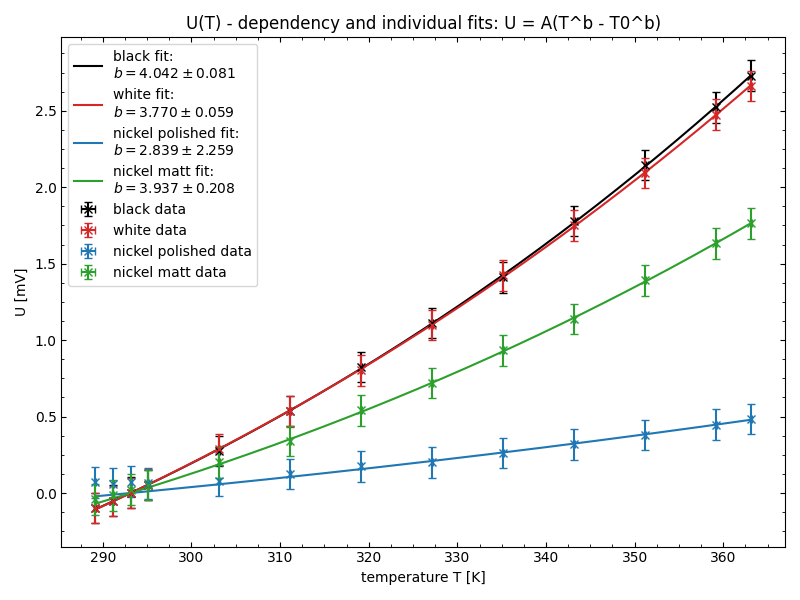
\includegraphics[width=0.5\textwidth]{../Images/individual_fits_U(T).png}
            \caption{Voltage generated by the thermopile as a function of the temperature of the cube for the different surfaces. The fit used is of the form $U = A (T^b - T_0^b)$. With $T_0 = 293.15 K$ as the reference temperature.}
            \label{fig:SBLeslie}
        \end{figure}

        As one can see in figure \ref{fig:SBLeslie} the black side emits the most thermal radiation and the polished nickel-plated side emits the least, which is expected since the black surface has the highest emissivity and the polished nickel-plated surface has the lowest emissivity. 
        The data of the polished nickel-plated surface is very noisy. This matches with it's fit exponent $b$ which is far off aswell, this will be discussed further below in more detail.

        \begin{table}[H]
            \centering
            \begin{tabular}{c|c}
                Surface & fit exponent $b$ \\
                \hline
                White & $3.770 \pm 0.059$ \\
                Black & $4.043 \pm 0.081$ \\
                Polished nickel-plated & $2.8 \pm 2.3$ \\
                Matte nickel-plated & $3.94 \pm 0.21$ \\
            \end{tabular}
            \caption{The exponents determined by the $U = A (T^b - T_0^b)$ fit to the data obtained by measurements on Leslie's cube.}
            \label{tab:SBLeslie}
        \end{table}
        The expected values of the exponents is $b=4$ according to the Stefan-Boltzmann law. The values obtained for the black and matte nickel-plated surfaces match that within their error, while the value obtained for the white and polished nickel-plated surface are a bit off.
        The value obtained for the white surface is close to the expected value, but the error is small enough to exclude $b=4$. The value obtained for the polished nickel-plated does match $b=4$ within the error, but the error is very large which is a good representation of the poor quality of the measurement. 
        This poor quality is due to the fact that the polished side reflects a lot of thermal radiation from the environment, which is also measured by the thermopile and can not be easily seperated from the radiation emitted by the surface itself. A solution to this would be to place the setup in a more contained environment and shield it further from external radiation. \\
        

